\documentclass{beamer}
\usepackage[utf8]{inputenc}

\usetheme{Madrid}
\usecolortheme{default}
\usepackage{amsmath,amssymb,amsfonts,amsthm}
\usepackage{txfonts}
\usepackage{tkz-euclide}
\usepackage{listings}
\usepackage{adjustbox}
\usepackage{array}
\usepackage{tabularx}
\usepackage{gvv}
\usepackage{lmodern}
\usepackage{circuitikz}
\usepackage{tikz}
\usepackage{graphicx}

\setbeamertemplate{page number in head/foot}[totalframenumber]

\usepackage{tcolorbox}
\tcbuselibrary{minted,breakable,xparse,skins}



\definecolor{bg}{gray}{0.95}
\DeclareTCBListing{mintedbox}{O{}m!O{}}{%
  breakable=true,
  listing engine=minted,
  listing only,
  minted language=#2,
  minted style=default,
  minted options={%
    linenos,
    gobble=0,
    breaklines=true,
    breakafter=,,
    fontsize=\small,
    numbersep=8pt,
    #1},
  boxsep=0pt,
  left skip=0pt,
  right skip=0pt,
  left=25pt,
  right=0pt,
  top=3pt,
  bottom=3pt,
  arc=5pt,
  leftrule=0pt,
  rightrule=0pt,
  bottomrule=2pt,

  colback=bg,
  colframe=orange!70,
  enhanced,
  overlay={%
    \begin{tcbclipinterior}
    \fill[orange!20!white] (frame.south west) rectangle ([xshift=20pt]frame.north west);
    \end{tcbclipinterior}},
  #3,
}
\lstset{
    language=C,
    basicstyle=\ttfamily\small,
    keywordstyle=\color{blue},
    stringstyle=\color{orange},
    commentstyle=\color{green!60!black},
    numbers=left,
    numberstyle=\tiny\color{gray},
    breaklines=true,
    showstringspaces=false,
}
%------------------------------------------------------------
%This block of code defines the information to appear in the
%Title page
\title %optional
{1.5.16}
\date{August  2025}
%\subtitle{A short story}

\author % (optional)
{J.NAVYASRI- EE25BTECH11028}

\begin{document}

\frame{\titlepage}
\begin{frame}{Question}
Find the  coordinates point \(A\) where  \(AB\) is a diameter of the circle with center \(=(3,-1)\) and point \(B=(2,6)\).
 
\end{frame}
 
\begin{frame}{given data}
 \[
\begin{tabular}[12pt]{ |c| c| c|} 
    \hline
    {Point} & {Vector} \\ 
    \hline
    B & $ \myvec{2 \\ 6} $  \\
    \hline
    P & $ \myvec{3 \\ -1} $   \\
    \hline  
    \end{tabular}
\]

   
\end{frame}

\begin{frame}{Theoretical Solution}

\underline{\textbf{Theory :}} Center of a circle is the mid-point of the diameter. \\

Let $P$ be the center of the given circle , with $AB$ as the diameter.

Let $\vec{A}$ be the Vector to be found 

\textit{Given :} 
\[
B \equiv \begin{pmatrix} 2 \\ 6 \end{pmatrix}, \quad P \equiv \begin{pmatrix} 3 \\ -1 \end{pmatrix}
\]
\end{frame}

\begin{frame}{Theoretical Solution}

Center of a circle is the mid point of the diameter. For a circle with center $\vec{P}$ and ends of diameters represented by vectors $\vec{A}$ and $\vec{B}$  
\[
\mathbf{P} = \frac{\mathbf{A} + \mathbf{B}}{2} \tag{0.1}
\]

Rearranging , we get:
\[
\mathbf{A} = 2\mathbf{P} - \mathbf{B} \tag{0.2}
\]
\end{frame}

\begin{frame}{Theoretical Solution}
Substituting the given vectors, we get:
\[
\mathbf{A} = 2 \begin{pmatrix} 3 \\ -1 \end{pmatrix} - \begin{pmatrix} 2 \\ 6 \end{pmatrix} \tag{0.3}
\]
\[
\mathbf{A} = \begin{pmatrix} 6 \\ -2 \end{pmatrix} - \begin{pmatrix} 2 \\ 6 \end{pmatrix} \tag{0.4}
\]
\[
\therefore \mathbf{A} \equiv \begin{pmatrix} 4 \\ -8 \end{pmatrix}
\]

\textbf{Hence , Coordinates of A are } 
\[
\begin{pmatrix} 4 \\ -8 \end{pmatrix}
\]
\end{frame}


\begin{frame}[fragile]
    \frametitle{C Code (1) - Function to find A matrix }

    \begin{lstlisting}

#include <stdio.h>
#include <math.h>
void func(double *P, double *B, double *A , int m )
{
    for ( int i = 0 ; i < m ; i++ )
    {
        A[i] = 2*P[i] - B[i] ; 
    }

}
    \end{lstlisting}
\end{frame}
\begin{frame}[fragile]
    \frametitle{C Code (1) - Function to Find Radius}

    \begin{lstlisting}

double radius(double *P , double *B , int m )
{
    double sum = 0.0; 
    for ( int i = 0 ; i < m ; i++ )
    {
        sum += pow(P[i]-B[i] , 2 );
    }
    return sqrt(sum) ; 
}

    \end{lstlisting}
\end{frame}


\begin{frame}[fragile]
    \frametitle{C Code (2) - Function to Generate Points on Circle}

    \begin{lstlisting}

#include <math.h>

void circle_gen(double *X , double *Y , double *P, int n , double r)
{
// n is no. of points to generates. x stores x coor , y stores y coor 
    for (int i  = 0 ; i < n ; i++ )
    {
        double theta = 2.0 * M_PI * i / n ; 
        X[i] = P[0] + r * cos(theta);
        Y[i] = P[1] + r * sin (theta); 
    }   
}
    \end{lstlisting}
\end{frame}
\begin{frame}[fragile]
    \frametitle{C Code (2) - Function to Generate Points on Line}

    \begin{lstlisting}
void line_gen (double *X, double *Y , double *A , double *B , int n , int m )
{
    double temp[m] ; 
    for (int i = 0 ; i < m ; i++)
    {
        temp [ i ] = (B[i]- A[i]) /(double) n ; 
    }
    for (int i = 0 ; i <= n ; i++ )
    {
        X[i] = A[0] + temp[0] * i ; 
        Y[i] = A[1] + temp[1] * i ;
    }
}

    \end{lstlisting}
\end{frame}
\begin{frame}[fragile]
    \frametitle{Python Code}
    \begin{lstlisting}
import ctypes
import numpy as np
import matplotlib.pyplot as plt

# Load shared C library
lib = ctypes.CDLL("./formula.so")

# Define argument and return types
lib.find_A.argtypes = [
    np.ctypeslib.ndpointer(dtype=np.float64, ndim=1, flags="C_CONTIGUOUS"),
    np.ctypeslib.ndpointer(dtype=np.float64, ndim=1, flags="C_CONTIGUOUS"),
    np.ctypeslib.ndpointer(dtype=np.float64, ndim=1, flags="C_CONTIGUOUS"),
]
lib.find_A.restype = None
\end{lstlisting}
\end{frame}

\begin{frame}[fragile]
    \frametitle{Python Code}
    \begin{lstlisting}
# Input vectors
P = np.array([3.0, -1.0], dtype=np.float64)
B = np.array([2.0, 6.0], dtype=np.float64)
A = np.zeros(2, dtype=np.float64)

# Call C function
lib.find_A(P, B, A)

print("A =", A)

# Plotting
fig, ax = plt.subplots()

# Circle parameters
center = P
radius = np.linalg.norm(A - P)  # radius = distance from center to A (or B)

\end{lstlisting}
\end{frame}

\begin{frame}[fragile]
    \frametitle{Python Code}
    \begin{lstlisting}
theta = np.linspace(0, 2*np.pi, 300)
x_circle = center[0] + radius*np.cos(theta)
y_circle = center[1] + radius*np.sin(theta)
ax.plot(x_circle, y_circle, 'b')

# Plot diameter line AB
ax.plot([A[0], B[0]], [A[1], B[1]], 'g--')

# Midpoint of AB for placing text "Diameter"
mid_x = (A[0] + B[0]) / 2
mid_y = (A[1] + B[1]) / 2
ax.text(mid_x + 0.5, mid_y + 0.5, "Diameter", color="green")
\end{lstlisting}
\end{frame}


\begin{frame}[fragile]
    \frametitle{Python Code}
    \begin{lstlisting}
# Mark points with coordinates
ax.scatter(*A, color='red')
ax.text(A[0]+0.3, A[1], f"A{tuple(A.astype(int))}")

ax.scatter(*B, color='red')
ax.text(B[0]+0.3, B[1], f"B{tuple(B.astype(int))}")

ax.scatter(*P, color='black')
ax.text(P[0]+0.3, P[1], f"P{tuple(P.astype(int))} (center)")

ax.set_aspect('equal')
ax.grid(True)
plt.show()
\end{lstlisting}
\end{frame}

\begin{frame}{Plot-Using Both C and Python}
    \centering
    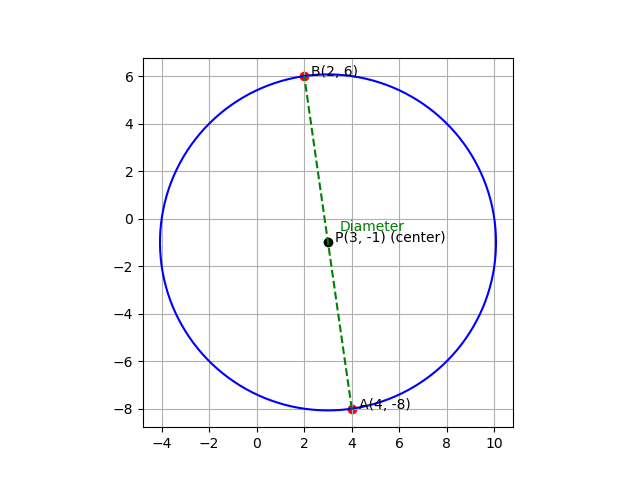
\includegraphics[width=\columnwidth, height=0.8\textheight, keepaspectratio]{figs/fig1.2.png}     
\end{frame}
\begin{frame}[fragile]
    \frametitle{Python Code}
    \begin{lstlisting}
import numpy as np
import matplotlib.pyplot as plt

P = np.array([2, 6])
B = np.array([3, -1])
A = 2*P - B

radius = np.linalg.norm(B - P)
theta = np.linspace(0, 2*np.pi, 300)
x_circle = P[0] + radius*np.cos(theta)
y_circle = P[1] + radius*np.sin(theta)
\end{lstlisting}
\end{frame}
\begin{frame}[fragile]
    \frametitle{Python Code}
    \begin{lstlisting}
plt.plot(x_circle, y_circle, 'r', label='Circle') 
plt.plot([A[0], B[0]], [A[1], B[1]], 'g--', label='Diameter')

plt.scatter([A[0], B[0], P[0]], [A[1], B[1], P[1]], color='blue')
plt.text(A[0], A[1]-0.5, f'A{tuple(A)}')
plt.text(B[0], B[1]+0.5, f'B{tuple(B)}')
plt.text(P[0]+0.2, P[1], f'P{tuple(P)}')
\end{lstlisting}
\end{frame}

\begin{frame}[fragile]
    \frametitle{Python Code}
    \begin{lstlisting}
  plt.axhline(0, color='black', linewidth=0.5)
plt.axvline(0, color='black', linewidth=0.5)
plt.grid(True)
plt.gca().set_aspect('equal', adjustable='box')

#  Legend moved to top-right corner
plt.legend(loc="upper right")

plt.xlabel("x")
plt.ylabel("y")
plt.title("Circle with Diameter AB and Center P")
plt.savefig("fig1.png")
plt.show()  
\end{lstlisting}
\end{frame}

\begin{frame}{Plot-Using  Python}
\textbf{Graph representation:}
\begin{figure}[H]
    \centering
 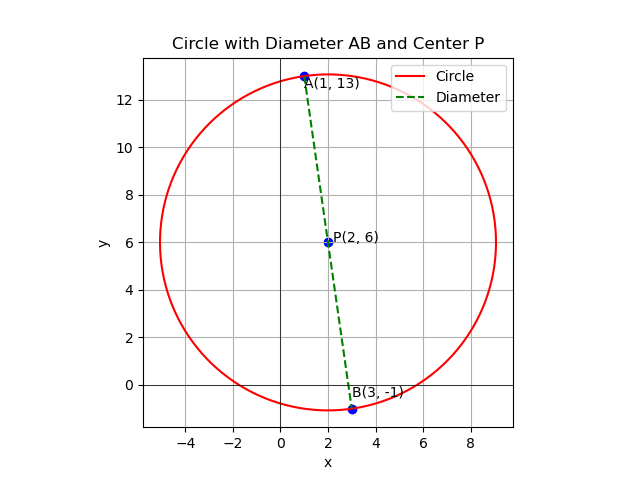
\includegraphics[width=0.5\linewidth]{figs/fig1.png}
    \caption{0}
    \label{fig:placeholder}
\end{figure}
\end{frame}

\end{document}